\documentclass{bioinfo}
\copyrightyear{2007}
\pubyear{2007}

% The default should be citep.
\renewcommand{\cite}{\citep}

\begin{document}
\firstpage{1}

\title[Rapid and accurate peptide identification]{Rapid and accurate
  peptide identification from tandem mass spectra}
\author[Park \textit{et~al}]{Christopher Park$^{\rm a}$,
Aaron Klammer$^{\rm b}$,
Lukas K\"{a}ll$^{\rm b}$, 
William S. Noble\,$^{\rm a,b,}$\footnote{To whom correspondence should be addressed}}
\address{
$^{\rm a}$Department of Computer Science and Engineering,
$^{\rm b}$Department of Genome Sciences, University of Washington,
  Seattle, WA, USA
}
\history{Received on XXXXX; revised on XXXXX; accepted on XXXXX}

\editor{Associate Editor: XXXXXXX}

\maketitle

\begin{abstract}
\section{Motivation:}  Mass spectrometry, the core technology in the
field of proteomics, promises to enable scientists to identify and
quantify the entire complement of proteins in a complex biological
sample.  Currently, the primary bottleneck in this type of experiment
is computational.  Existing algorithms for interpreting mass spectra
are slow and fail to identify a large proportion of the given spectra.

\section{Results:} We describe a database search program called Crux
that extends the state of the art in peptide identification in several
significant respects.  Crux reimplements and extends the widely used
database search program SEQUEST.  For speed, Crux uses a peptide
indexing scheme to rapidly retrieve candidate peptides for a given
spectrum.  For each peptide in the target database, Crux generates
shuffled decoy peptides on the fly, providing a good null model and,
hence, accurate false discovery rate estimates.  In a second analysis
stage, Crux trains a machine learning model to discriminate between
target and decoy peptides, thereby significantly improving the overall
rate of peptide identification.

\section{Availability:}
\href{http://noble.gs.washington.edu/proj/crux}{http://noble.gs.washington.edu/proj/crux}
\section{Contact:} \href{noble@gs.washington.edu}{noble@gs.washington.edu}
\end{abstract}

\section{Introduction}

Tandem mass spectrometry is the method of choice for many protein
identification studies.  However, this technology suffers from an
analysis bottleneck, with a need for more efficient and more accurate
methods of mapping from the observed fragmentation spectra to the
corresponding peptides.

The most widely used methods for peptide identification, such as
SEQUEST \cite{eng:approach}, MASCOT \cite{perkins:probability},
X!Tandem \cite{craig:tandem} and Inspect \cite{tanner:inspect},
exploit a database of known protein sequences.  For each observed
spectrum, these methods search the database for the peptide whose
theoretical spectrum best matches the observed spectrum.  The
resulting peptide-spectrum matches (PSMs) can be ranked using a
pre-defined score function, or by using machine learning methods such
as linear discriminant analysis \cite{keller:empirical}, support
vector machines \cite{anderson:new, kall:semi-supervised} or decision
trees \cite{elias:intensity}.

\begin{figure*}
\centering
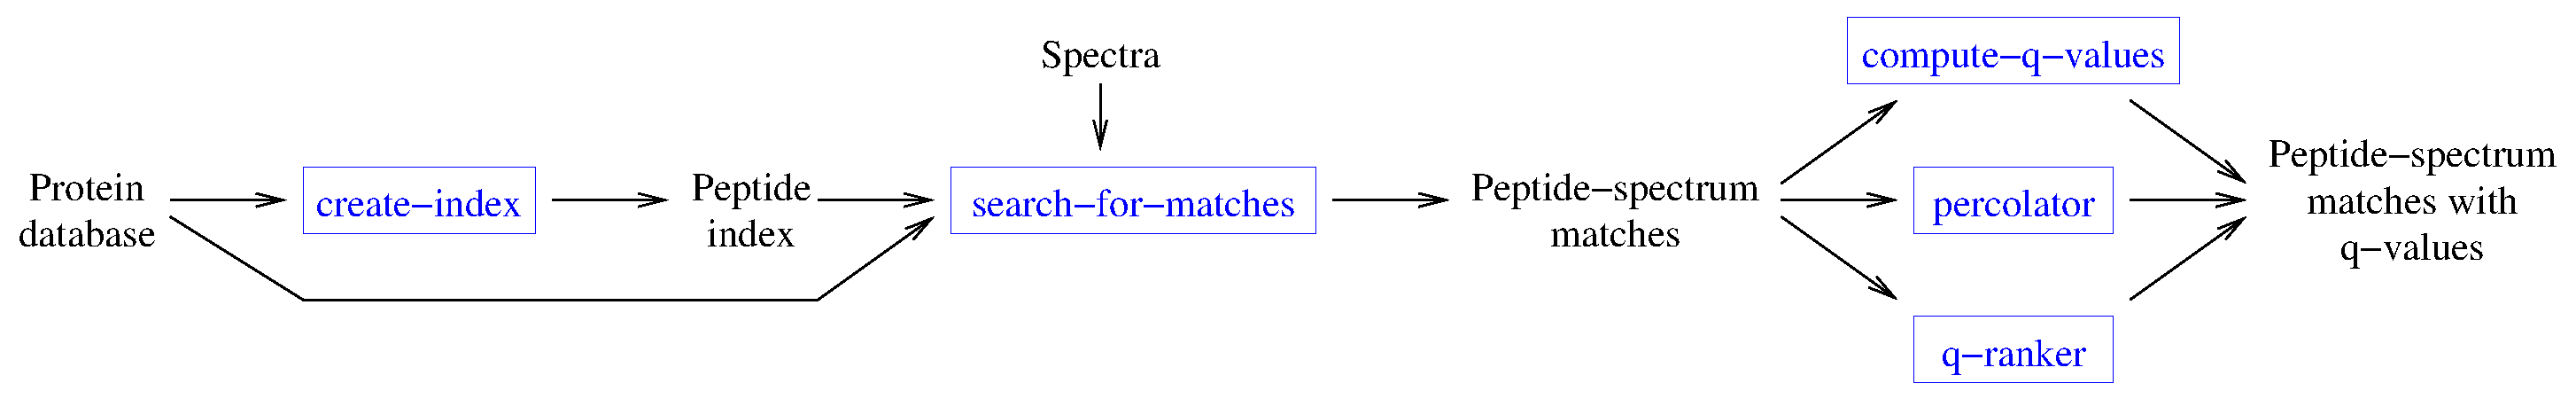
\includegraphics[width=6.5in]{schematic.eps}
\caption{{\bf The Crux algorithm.}  Crux takes as input a collection
  of fragmentation spectra and a target protein sequence database, and
  produces a list of peptide-spectrum matches, each with an associated
  $q$-value.
  \label{figure:crux}}
\end{figure*}

In this work, we describe a computational tool called Crux that solves
the peptide identification problem efficiently and accurately.  As
illustrated in Figure~\ref{figure:crux}, Crux incorporates a rapid
peptide lookup scheme, a static scoring system for relative ranking of
peptides with respect to each spectrum, a null model based on a decoy
database of shuffled peptides generated on the fly, and a dynamically
trained support vector machine for ranking the complete collection of
PSMs.  Relative to the current state of the art, Crux makes the
following primary contributions:

\begin{itemize}

\item {\bf Efficient retrieval of candidate peptides.}  Given a
  spectrum with a specified precursor mass-to-charge ratio (m/z), Crux
  uses a precomputed peptide database to retrieve efficiently all
  peptides whose m/z lies within a user-specified window around the
  target m/z (called {\em candidate peptides}).  The database is
  sorted by peptide mass and is stored on disk, with mass indices
  stored in memory.  We show that, relative to SEQUEST's strategy of
  reading the protein sequence database from disk for each new
  spectrum, the indexed database decreases search time by X\% on
  average.

\item {\bf On-the-fly generation of decoy peptides.}  In evaluating
  the statistical significance of a PSM, mass spectrometrists
  frequently employ a {\em decoy database} comprised of protein
  sequences that have been reversed, shuffled or generated from a
  Markov chain derived from the given {\em target database}.  The
  number of matches to the decoy database yields an estimate of the
  false discovery rate associated with a collection of target PSMs.
  Crux uses this target-decoy strategy, generating decoys by shuffling
  the target peptides.  This approach ensures that each decoy peptide
  exhibits precisely the same amino acid composition and total mass as
  the corresponding target decoy.  To avoid the memory overhead
  associated with storing shuffled, non-overlapping decoy peptides in
  memory, Crux generates decoy peptides on the fly.

\item {\bf Dynamically trained PSM scoring function.}  After scoring
  all peptides with respect to a given spectrum, the top-ranked PSM
  must be ranked with respect to other PSMs from the same data set.
  Some score functions, such as SEQUEST's cross-correlation score
  (XCorr), have been used to carry out both relative ranking and
  absolute ranking; however, numerous studies have demonstrated that
  better absolute rankings can be achieved by using machine learning
  methods \cite{keller:empirical, anderson:new, elias:intensity,
  kall:semi-supervised}.  Crux incorporates a recently described
  method, called Percolator, for training a machine learning method to
  discriminate between target and decoy PSMs.  This dynamically
  trained model incorporates specific characteristics of the given
  data set.  Furthermore, Crux's implementation of Percolator allows
  the user to include the observed and predicted liquid chromatography
  retention time \cite{klammer:effect} as an additional feature.

\item {\bf Accurate false discovery rate estimates.}  Crux uses
  well-established statistical methods to estimate false discovery
  rates based upon decoy PSMs \cite{benjamini:controlling}.  To avoid
  biasing the estimates, separate sets of decoy PSMs are used to train
  the machine learning method and to estimate the final false
  discovery rate.  Crux reports, along with each PSM, a $q$-value,
  which is defined as the minimal false discovery rate threshold at
  which a given PSM is deemed correct \cite{storey:statistical}.

\end{itemize}

Perhaps most significantly, from the perspective of the mass
spectrometry research community, Crux provides all of the above in a
single stand-alone C program which is distributed, with source code,
free for academic use.  Below, we demonstrate that Crux is both
efficient and accurate, yielding FIXME.

\section{Approach}

\subsection{Rapid retrieval of candidate peptides}

When presented with a new query spectrum and its associated precursor
mass, Crux must first retrieve from the sequence database all of the
candidate peptides, i.e., peptides whose masses lie within a specified
range of the precursor mass.  A straightforward retrieval method is to
read the entire database from disk for each query, evaluating
candidate peptides as they are encountered.  This approach, which is
used by SEQUEST, is space-efficient but can be slow for large
databases.

In addition to implementing the above approach, Crux offers an
alternative strategy that allows for more efficient candidate peptide
retrieval.  In this approach, the user must pre-process a given
protein database to produce a binary protein database and a binary
peptide index.  The pre-processing step sorts all of the peptides in
the database by mass and stores pointers to their locations in the
protein database (sequence index, start position, and peptide length).
Crux can then quickly retrieve a set of candidate peptides via a
simple range query on the peptide index.

Upon execution, Crux accesses the binary protein database and the
peptide index as memory-mapped files.  This approach offloads to the
operating system the decision about how much of the database to store
in memory, ensuring that small databases are read fully into memory
but large databases are paged into and out of memory only as needed.

\subsection{Scoring peptide-spectrum matches}

After retrieving all of the candidate peptides for a given spectrum,
Crux follows the strategy used by SEQUEST.  Initially, the candidate
peptides are ranked according to the preliminary SEQUEST score $Sp$.
Subsequently, the 500 top-scoring peptides are re-ranked according to
the cross-correlation score $XCorr$.

For $Sp$ scoring, Crux applies several pre-processing steps to the
observed spectrum.  First, Crux takes the square root of each peak's
intensity and rounds each peak's m/z to the nearest integer.  Second,
Crux normalize the peak intensities to sum to 100.  Third, Crux
extracts the top 200 highest intensity peaks.  Crux compares the
resulting observed spectrum with the b and y fragment ions from the
candidate peptide to compute $Sp$ as follows:
\[
\mbox{FIXME: Insert equation here}
\]

$Xcorr$ scoring also requires some pre-processing of the observed
spectrum.  As before, First, Crux takes the square root of each peak's
intensity and rounds each peak's m/z to the nearest integer.  Second,
Crux divides the spectrum into 10 regions and normalizes the spectrum
intensity in each region to maximum 50.0. To create the theoretical
spectrum from the candidate peptide, Crux constructs a spectrum with
peak intensity 50.0 for b and y ions, 25.0 for the +/- 1 m/z flanking
peaks of each b and y ion, and 10.0 for ions resulting from a neutral
loss of ammonia from b or y ions or neutral loss of water
from b ions.  Crux then computes $Xcorr$ as follows:
\[
\mbox{FIXME: Insert equation here}
\]

\subsection{Null peptide generation}

When identifying peptides from tandem mass spectra, a commonly used
null model is to search the given set of spectra against a {\em decoy
database}.  A decoy database is a database of amino acid sequences
that is derived from the original protein database (called the {\em
target database}) by reversing the target sequences
\cite{moore:qscore}, shuffling the target sequences
\cite{klammer:effects}, or generating the decoy sequences at random
using a Markov model with parameters derived from the target sequences
\cite{colinge:olav}.  Ideally, the decoy database should contain
peptide-like amino acid sequences that are not in the target database.

Crux uses a decoy strategy; however, rather than generating a fixed
decoy database, Crux generates decoys on the fly.  For each
computation of $Sp$ or $Xcorr$ between a spectrum and a target
peptide, Crux generates a corresponding decoy peptide by shuffling the
non-terminal amino acids of the target peptide.  Consequently, Crux
reports for every target PSM a corresponding decoy PSM.  The decoy PSM
score distribution is used during Percolator training
(Section~\ref{section:percolator}) and to estimate $q$~values
(Section~\ref{section:q-value}).  On-the-fly decoy generation
introduces a small computational overhead but saves space, because the
decoy database does not need to be stored.  Optionally, Crux can
report multiple decoys per target.

\subsection{Percolator}
\label{section:percolator}

Identifying peptides from tandem mass spectra via database search is,
fundamentally, a ranking procedure, in which good PSMs are ranked
above poor PSMs.  Furthermore, this ranking task can be usefully
separated into two phases: a {\em relative ranking} task, in which all
of the peptides in the database are ranking relative to a single
spectrum to identify a single best PSM for that spectrum, and an {\em
absolute ranking} task, in which the top-ranked PSMs for multiple
spectra are ranked relative to one another.  Absolute ranking is, by
definition, more difficult than relative ranking.

Empirical evidence suggests that, although $Xcorr$ does a good job at
relative ranking, it performs more poorly when attempting to rank PSMs
absolutely \cite{keller:empirical, anderson:new}.  We therefore employ
a semi-supervised machine learning method to learn dynamically an
absolute PSM ranking function \cite{kall:semi-supervised}.  A subset
of the high-scoring target PSMs is used as positive examples, and all
of the decoy PSMs are used as negative examples to train a
discriminative classification algorithm called a support vector
machine (SVM) \cite{boser:training, noble:what}.  Each PSM is
characterized using a collection of features that capture
characteristics of the spectrum, the peptide, and the quality of the
match between the spectrum and the peptide.  Details of this
semi-supervised learning algorithm, called Percolator, are given in
\citet{kall:semi-supervised}.

Crux implements the Percolator algorithm, using half of the computed
decoy PSMs to train the absolute scoring function.  The remaining
decoy PSMs are reserved for estimate $q$~values, as described next.

\subsection{$q$~value estimation}
\label{section:q-value}

Crux produces as output a ranked list of target PSMs, one per spectrum
in the given data set.  Along with each PSM, Crux reports a $q$~value,
which is defined as the minimal false discovery rate at which this PSM
is called positive \cite{storey:statistical}.  False discovery rates
are estimated using the method of \cite{benjamini:controlling}, with
$p$~values defined using decoy PSMs scored using the Percolator score
function.

\begin{methods}
\section{Methods}

All experiments were performed on a RedHat Linux machine with an
Athlon MP 2000, 2 x 1.67 GHz processor and 2~GB of RAM.

Using Crux, we precomputed a peptide database for tryptic peptides of
length 6--50 amino acids while allowing missed cleavage sites in the
non-redundant protein database (06/02/2007, 3,292,818 proteins). This
procedure required 19~hours and 14~GB of disk space.

We use the following publicly available tandem mass spectrometry data
sets.  FIXME

\end{methods}

\section{Results}

\subsection{Accurate reimplementations of $Sp$ and $Xcorr$}

\begin{figure*}
  \centering
  \begin{tabular}{cc}
    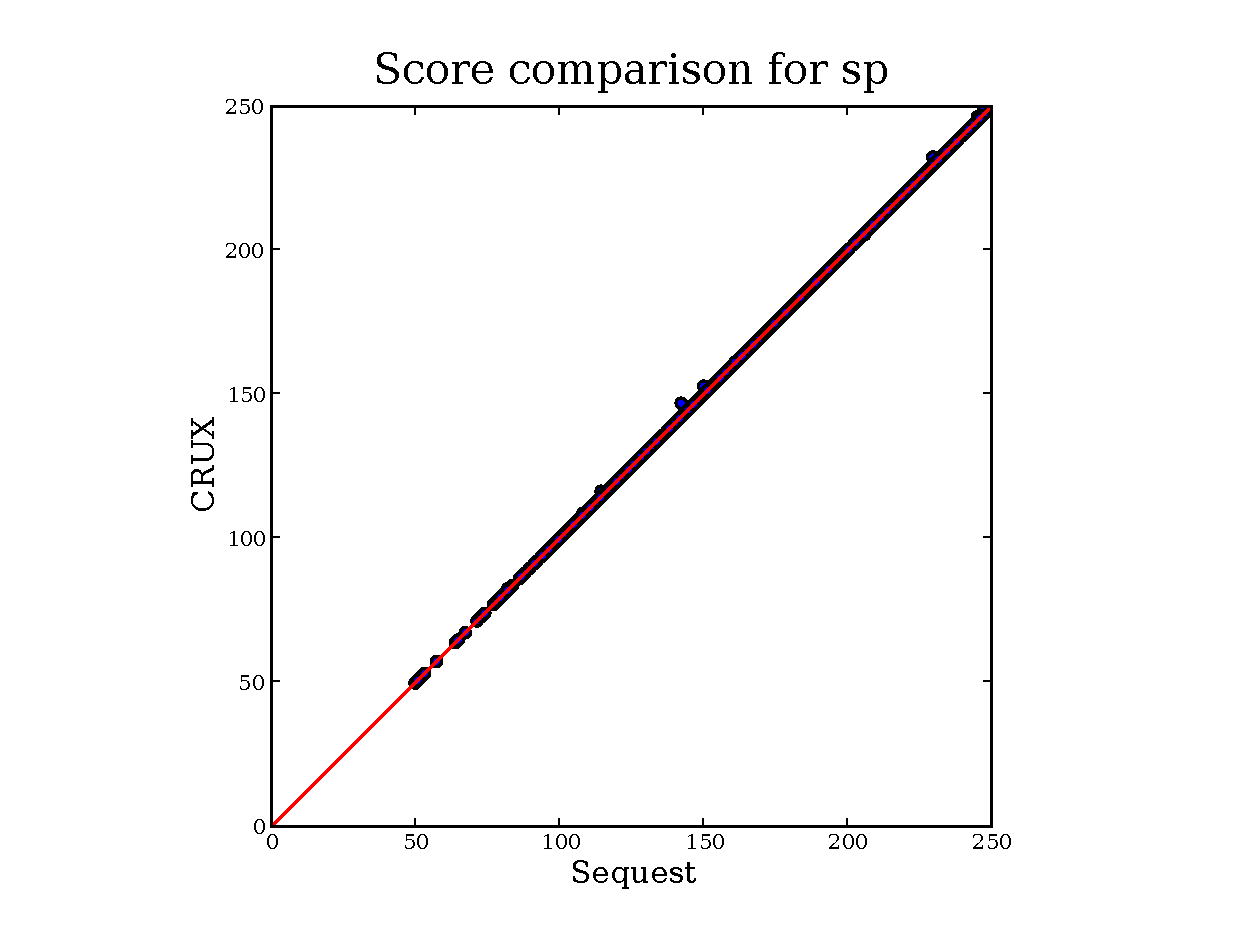
\includegraphics[width=3in]{./Images/random-sp.eps} &
    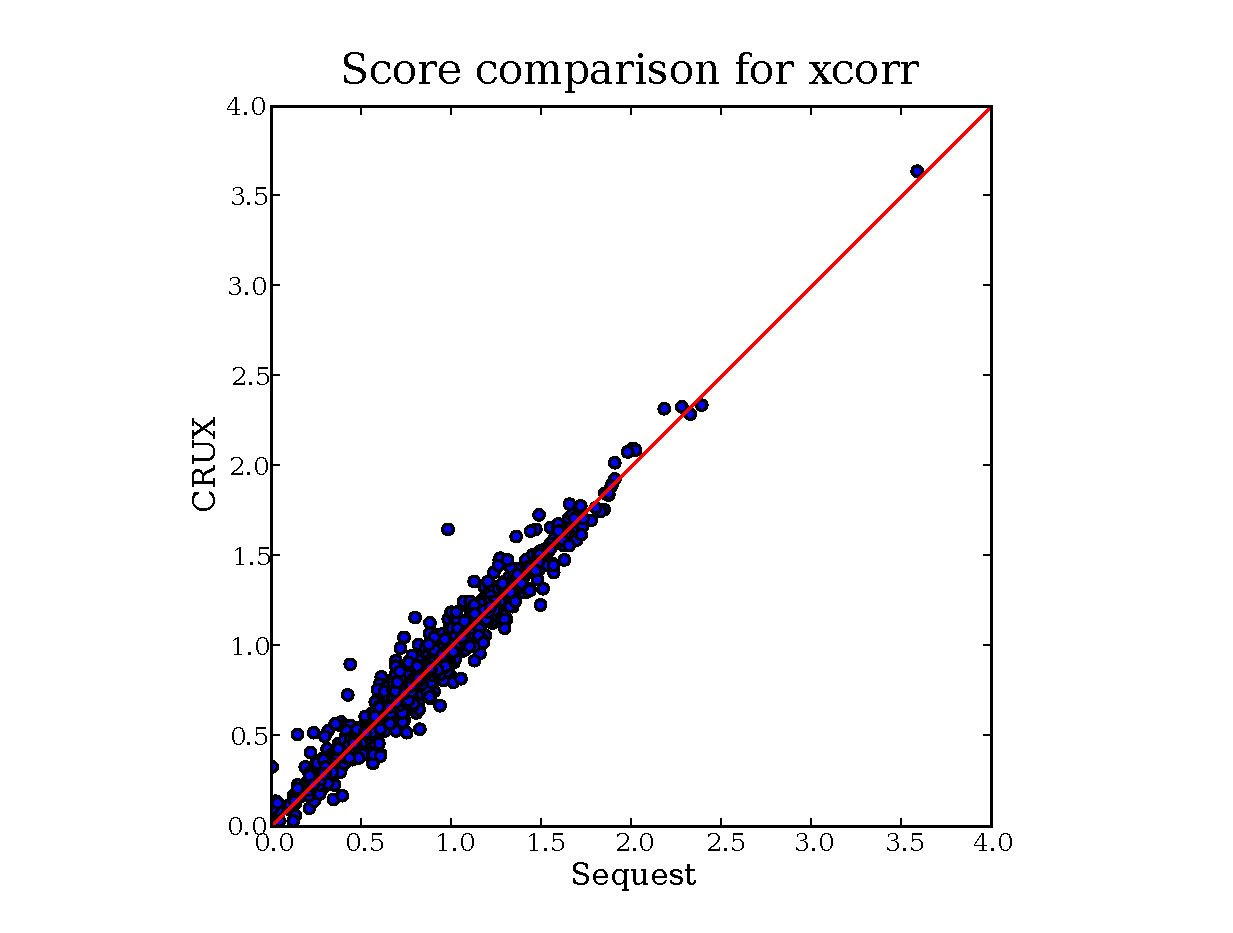
\includegraphics[width=3in]{./Images/random-xcorr.eps} \\
  A & B \\
  \end{tabular}
  \caption{{\bf Re-implementation of Sp and Xcorr scoring functions.}
  The figure plots, for a collection of peptide-spectrum matches, the
  Sp (A) and XCorr (B) scores as computed by Crux as a function of the
  same scores as computed by SEQUEST.
  \label{figure:sp-xcorr}}
\end{figure*}

SEQUEST is the first and one of the most widely used database search
methods for peptide identification from tandem mass spectra.  We
wanted to begin with a reimplementation of the core of SEQUEST, which
is the $Sp$ and $Xcorr$ score functions.  Figure~\ref{figure:sp-xcorr}
plots the Crux-calculated versions of these scores as a function of
the SEQUEST-calculated versions of these scores.  The figure shows
that the vast majority of the PSMs receive identical scores using
either method.  Among a collection of FIXME spectra, searched with a
mass window of FIXME m/z, the top-ranked peptide according to Crux
differs from the top-ranked peptide according to SEQUEST in only FIXME
cases.  

\subsection{Efficient retrieval of candidate peptides}

\begin{figure}
  \centering
  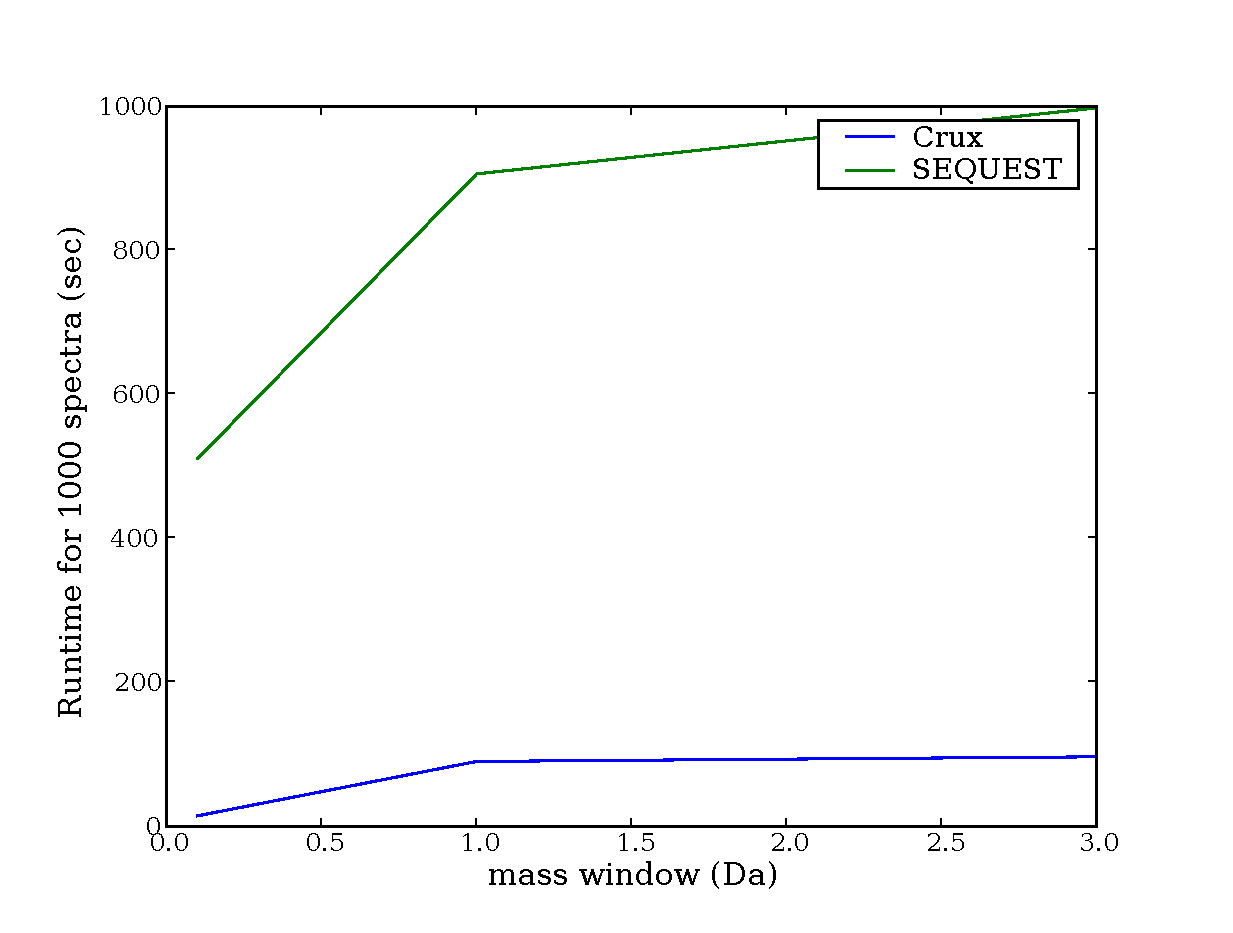
\includegraphics[width=3in]{./Images/indexing.eps}
  \caption{{\bf Rapid database searching.}  The figure plots the total
  running time required to search 10,000 tandem mass spectra against
  the non-redundant protein database, plotted as a function of the m/z
  tolerance used to define candidate peptides.  The two series
  correspond to searching with SEQUEST and searching with Crux.  For
  purposes of comparison, Crux's decoy searching and the Percolator
  post-processor are turned off.
  \label{figure:indexing}}
\end{figure}

To demonstrate the efficiency of Crux's candidate peptide retrieval
strategy, we searched with a collection of 100 spectra against the
NRDB, generating candidate peptides from a series of increasing wider
m/z windows.  Figure~\ref{figure:indexing} plots the search time as a
function of m/z window width.  For this experiment, we use a modified
version of SEQUEST that only computes Sp (and not XCorr), and we
compare its running time to that of Crux running in the same fashion.
As expected, Crux runs more quickly than SEQUEST, because Crux does
not need to scan the entire database to retrieve a small collection of
candidate peptides.  The difference is most pronounced when the mass
tolerance window is small.  For example, with a mass tolerance window
of 0.1, SEQUEST requires 3.5~hrs clock time, whereas Crux requires
0.1~hrs.  This represents a 35-fold improvement.  However, even when
we use a mass tolerance of 3, Crux yields a six-fold speed improvement
(0.6~hours versus 3.6~hours).

\subsection{Improved identification of peptides}

\begin{figure}
\centering
Insert figure here
\caption{{\bf Improved peptide identification.}  The figure plots, for
  a variety of database search algorithms, the number of PSMs as a
  function of the estimated $q$~value.  The five series correspond to
  SEQUEST, Crux's implementation of SEQUEST using a shuffled decoy
  database, Crux using decoys generated on-the-fly, Crux with the
  Percolator post-processor enabled, and Crux with Percolator,
  including retention time features.
  \label{figure:pq-plot}}
\end{figure}

\section{Discussion}

The peptide index can be extended to allow for
storage of additional useful pieces of pre-computed information: 
e.g.  predicted peak intensities, predicted peptide retention time,
or peptide proteotypicity.  % probably not a word!

% N.B. We should make sure to mention the file-handle limit at some point.

\section*{Funding}

\section*{Acknowledgment}

% Mention Ting Chen's contribution

% We thank Grant and Tobias Mann for helpful advice. Funding:
% NIH grants U01~HG003161 and R01~GM071923.



% N.B. To use the bibliography, check out the 'refs' CVS module and add it to
% your Bibtex path.

\bibliographystyle{plainnat}
\bibliography{refs} 

\end{document}
